\lecture{1}{}{Introduction to State-Space Dynamics}

\subsection{Continuous-Time Dynamics}

Welcome to the first lecture on Optimal Control! Today we will begin our journey by formalizing the concept of a dynamical system. The core idea is to represent the evolution of a system over time using a mathematical model.

\begin{definition}[State-Space Representation]
	A general continuous-time smooth dynamical system can be described by a first-order ordinary differential equation (ODE) of the form:
	\begin{equation}
		\dot{\vec{x}}(t) = f(\vec{x}(t), \vec{u}(t), t)
		\label{eq:general_dynamics}
	\end{equation}
	where:
	\begin{itemize}
		\item \(\vec{x}(t) \in \mathbb{R}^n\) is the \textbf{state vector} of the system at time \(t\). It is a complete summary of the system's history, meaning that the state at time \(t\) is sufficient to predict the future evolution of the system given the future inputs.
		\item \(\vec{u}(t) \in \mathbb{R}^m\) is the \textbf{input vector} (or control vector) at time \(t\). These are the external signals we can manipulate to influence the system's behavior.
		\item \(f: \mathbb{R}^n \times \mathbb{R}^m \times \mathbb{R} \to \mathbb{R}^n\) is a smooth function called the \textbf{dynamics function} or vector field. It maps the current state, input, and time to the time derivative of the state.
	\end{itemize}
\end{definition}

For many systems, especially mechanical ones, the state vector \(\vec{x}\) has a specific structure. It's often composed of the system's configuration and its velocity.

\begin{notation}
	For a mechanical system, we typically define the state as:
	\[
		\vec{x} = \begin{bmatrix} \vec{q} \\ \vec{v} \end{bmatrix}
	\]
	where \(\vec{q}\) is the \textbf{configuration} or "pose" of the system, and \(\vec{v}\) is its corresponding \textbf{velocity}. Note that the configuration space is not always a simple vector space like \(\mathbb{R}^k\); it can be a more complex manifold, like a circle \(S^1\) or the special orthogonal group \(SO(3)\) for rotations.
\end{notation}

\begin{eg}[The Simple Pendulum]
	Let's consider a simple pendulum, which consists of a point mass \(m\) attached to a massless rod of length \(l\), pivoting frictionlessly. A torque \(\tau\) can be applied at the pivot.

	\begin{center}
		% include the pendulum figure
		% Figures/pendulum.tex
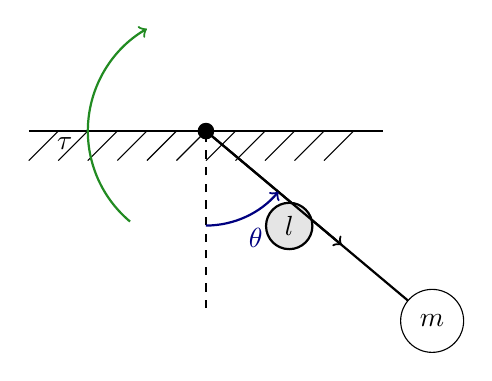
\begin{tikzpicture}[scale=1.5]
    % Support
    \draw[thick] (-1.5, 0) -- (1.5, 0);
    \foreach \i in {-1.25,-1,...,1.25} {
            \draw (\i, 0) -- (\i-0.25, -0.25);
        }

    % Pivot
    \fill[black] (0,0) circle (2pt);

    % Pendulum
    \def\angle{-40}
    \def\len{2.5}
    \draw[thick] (0,0) -- (\angle:\len) node[circle, draw, fill=gray!20, midway, left=2pt] {$l$};

    % Mass
    \node[circle, draw, fill=white, minimum size=0.8cm] (mass) at (\angle:\len) {$m$};

    % Angle
    \draw[->, dashed] (0,-1.5) -- (0,0);
    \draw[->, thick] (0,0) -- (\angle:1.5);
    \draw[->, thick, ForestGreen] (\angle-90:1) arc (\angle-90:\angle-200:1);
    \node at (\angle-135:1.2) {$\tau$};

    % Angle arc
    \draw[->, thick, NavyBlue] (0,0) ++(-90:0.8) arc (-90:\angle:0.8);
    \node[NavyBlue] at (-65:1) {$\theta$};
\end{tikzpicture}
	\end{center}

	The equation of motion for this system can be derived from Newton's second law for rotation, \(\sum \tau = I\alpha\), where \(I = ml^2\) is the moment of inertia and \(\alpha = \ddot{\theta}\) is the angular acceleration. The torques acting on the mass are the applied torque \(\tau\) and the torque due to gravity, \(-mgl\sin(\theta)\). This gives us:
	\begin{equation}
		ml^2 \ddot{\theta} + mgl\sin(\theta) = \tau
		\label{eq:pendulum_eom}
	\end{equation}
	To put this into our state-space form, we define our state and input:
	\begin{itemize}
		\item Configuration: \(q = \theta \in S^1\) (the space of angles, a circle)
		\item Velocity: \(v = \dot{\theta} \in \mathbb{R}\)
		\item State: \(\vec{x} = \begin{bmatrix} \theta \\ \dot{\theta} \end{bmatrix} \in S^1 \times \mathbb{R}\) (a cylinder)
		\item Input: \(u = \tau \in \mathbb{R}\)
	\end{itemize}
	Now we can write the dynamics \(\dot{\vec{x}} = f(\vec{x}, u)\):
	\[
		\dot{\vec{x}} = \dv{t} \begin{bmatrix} \theta \\ \dot{\theta} \end{bmatrix} = \begin{bmatrix} \dot{\theta} \\ \ddot{\theta} \end{bmatrix}
	\]
	From \autoref{eq:pendulum_eom}, we can solve for \(\ddot{\theta}\):
	\[
		\ddot{\theta} = \frac{1}{ml^2}(\tau - mgl\sin(\theta))
	\]
	Substituting this back, we get the state-space representation:
	\begin{equation}
		\dot{\vec{x}} = f(\vec{x}, u) = \begin{bmatrix} x_2 \\ \frac{1}{ml^2}(u - mgl\sin(x_1)) \end{bmatrix}
		\label{eq:pendulum_ss}
	\end{equation}
	where we have used \(x_1 = \theta\) and \(x_2 = \dot{\theta}\).
\end{eg}


\subsection{Control-Affine Systems}

A very common and important class of nonlinear systems are those that are "affine" in the control input.

\begin{definition}[Control-Affine System]
	A system is called \textbf{control-affine} if its dynamics can be written in the form:
	\begin{equation}
		\dot{\vec{x}} = f_0(\vec{x}) + B(\vec{x})\vec{u}
	\end{equation}
	Here, \(f_0(\vec{x})\) is called the \textbf{drift vector field}, representing the system's natural dynamics when no control is applied. The matrix \(B(\vec{x})\) is the \textbf{input Jacobian}, which describes how the control input \(\vec{u}\) affects the state's velocity at a given state \(\vec{x}\).
\end{definition}

\begin{note}
	Most mechanical systems can be expressed in this form. For our pendulum example \autoref{eq:pendulum_ss}, we can separate the terms to see its control-affine structure:
	\[
		\dot{\vec{x}} = \underbrace{\begin{bmatrix} x_2 \\ -\frac{g}{l}\sin(x_1) \end{bmatrix}}_{f_0(\vec{x})} + \underbrace{\begin{bmatrix} 0 \\ \frac{1}{ml^2} \end{bmatrix}}_{B(\vec{x})} u
	\]
	Notice that in this case, the input Jacobian \(B\) is constant.
\end{note}


\subsection{Manipulator Dynamics and Euler-Lagrange}

The dynamics of robotic manipulators (and mechanical systems in general) have a well-defined structure.

\begin{theorem}[Manipulator Equation]
	The dynamics of a fully-actuated mechanical system can be written as:
	\begin{equation}
		\mat{M}(\vec{q})\ddot{\vec{q}} + \mat{C}(\vec{q}, \dot{\vec{q}})\dot{\vec{q}} + \vec{g}(\vec{q}) = \mat{B}(\vec{q})\vec{u} + \vec{\tau}_{ext}
		\label{eq:manipulator}
	\end{equation}
	where:
	\begin{itemize}
		\item \(\mat{M}(\vec{q})\) is the symmetric, positive-definite \textbf{mass matrix}.
		\item \(\mat{C}(\vec{q}, \dot{\vec{q}})\dot{\vec{q}}\) represents Coriolis and centrifugal forces.
		\item \(\vec{g}(\vec{q})\) is the vector of gravitational forces.
		\item \(\mat{B}(\vec{q})\) is the input mapping, and \(\vec{\tau}_{ext}\) are other external forces.
	\end{itemize}
	This is a second-order ODE. To convert it to a first-order state-space form, we can again let \(\vec{x} = [\vec{q}^{\top}, \dot{\vec{q}}^{\top}]^{\top}\). Then:
	\[
		\dot{\vec{x}} = \begin{bmatrix} \dot{\vec{q}} \\ \mat{M}(\vec{q})^{-1} (\mat{B}(\vec{q})\vec{u} + \vec{\tau}_{ext} - \mat{C}(\vec{q}, \dot{\vec{q}})\dot{\vec{q}} - \vec{g}(\vec{q})) \end{bmatrix}
	\]
	This is also in the control-affine form.
\end{theorem}

\begin{intuition}
	This structured form is not arbitrary; it is a direct consequence of the Euler-Lagrange equations from classical mechanics. The Lagrangian \(\mathcal{L}\) of a system is defined as the difference between its kinetic energy \(T\) and potential energy \(U\):
	\[
		\mathcal{L}(\vec{q}, \dot{\vec{q}}) = T(\vec{q}, \dot{\vec{q}}) - U(\vec{q})
	\]
	For mechanical systems, the kinetic energy is \(T = \frac{1}{2}\dot{\vec{q}}^{\top} \mat{M}(\vec{q})\dot{\vec{q}}\). The Euler-Lagrange equation then gives the dynamics:
	\[
		\dv{t}\left(\pdv{\mathcal{L}}{\dot{\vec{q}}}\right) - \pdv{\mathcal{L}}{\vec{q}} = \vec{\tau}_{\text{gen}}
	\]
	where \(\vec{\tau}_{\text{gen}}\) are the generalized forces acting on the system (like control inputs and external forces). Working through this derivation yields the manipulator  \autoref{eq:manipulator}.
\end{intuition}

\subsection{Linear Systems}

A particularly simple yet powerful class of systems are linear systems.

\begin{definition}[Linear Time-Varying System]
	A system is linear if its dynamics can be written as:
	\begin{equation}
		\dot{\vec{x}}(t) = \mat{A}(t)\vec{x}(t) + \mat{B}(t)\vec{u}(t)
	\end{equation}
	If the matrices \(\mat{A}\) and \(\mat{B}\) are constant, the system is called \textbf{Linear Time-Invariant (LTI)}.
	\[
		\dot{\vec{x}} = \mat{A}\vec{x} + \mat{B}\vec{u}
	\]
\end{definition}

Linear systems are fundamental in control theory, not just because they are easy to analyze, but because they can serve as local approximations of nonlinear systems.

\begin{prev}
	We can linearize a nonlinear system \(\dot{\vec{x}} = f(\vec{x}, \vec{u})\) around a nominal trajectory \((\bar{\vec{x}}(t), \bar{\vec{u}}(t))\). Let \(\delta\vec{x} = \vec{x} - \bar{\vec{x}}\) and \(\delta\vec{u} = \vec{u} - \bar{\vec{u}}\). A first-order Taylor expansion gives:
	\[
		\dot{\bar{\vec{x}}} + \delta\dot{\vec{x}} \approx f(\bar{\vec{x}}, \bar{\vec{u}}) + \underbrace{\left.\pdv{f}{\vec{x}}\right\vert_{\bar{\vec{x}}, \bar{\vec{u}}}}_{\mat{A}(t)} \delta\vec{x} + \underbrace{\left.\pdv{f}{\vec{u}}\right\vert_{\bar{\vec{x}}, \bar{\vec{u}}}}_{\mat{B}(t)} \delta\vec{u}
	\]
	Since \(\dot{\bar{\vec{x}}} = f(\bar{\vec{x}}, \bar{\vec{u}})\) (it's a valid trajectory), the dynamics of the error \(\delta\vec{x}\) are approximately linear:
	\[
		\delta\dot{\vec{x}} \approx \mat{A}(t)\delta\vec{x} + \mat{B}(t)\delta\vec{u}
	\]
	This process of linearization is a cornerstone of control design for nonlinear systems, and we will revisit it many times in this course.
\end{prev}
\newpage
